\section{Konzept}
Ausgehend von unseren Rechercheergebnissen haben wir unseren Fuchsjagd-Sender
folgendermaßen konzipiert.
\subsection{Versorgung}
\begin{figure}[H]
    \centering
    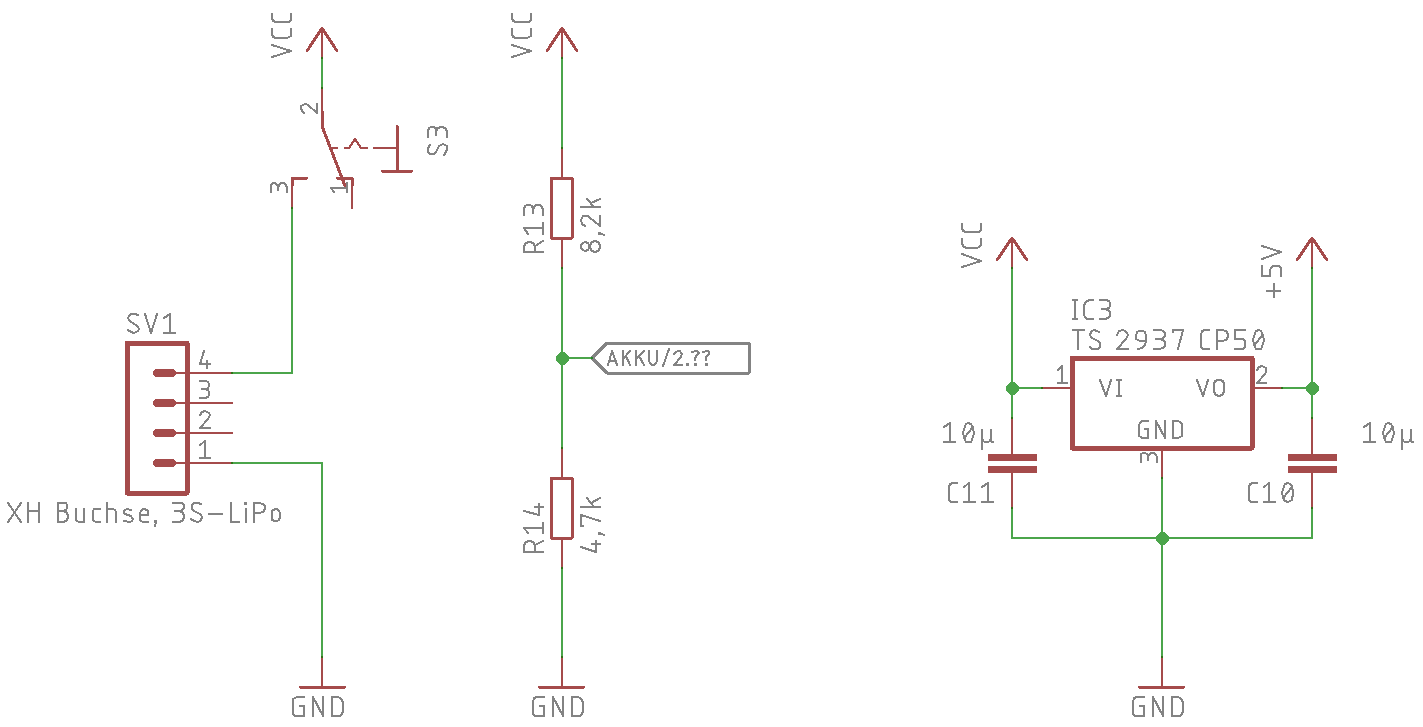
\includegraphics{res/Versorgung.png}
    \caption{Versorgung der Platine}
\end{figure}
Die Platine wird über einen dreizelligen Lithium-Ionen-Akku mit einer üblichen Nennspannung
von $11,1$V betrieben. Da unter anderem der Mikrocontroller nur mit $5$V versorgt
werden kann, nutzen wie einen Linearregler, der zusätzlich zu $12$V Schiene eine
$5$V Schiene erzeugt.

\subsection{Filterung des erzeugten Signals}
Damit der Sender ausschließlich im erlaubten Band sendet, wird der Verstärkerstufe
ein Tiefpassfilter nachgeschaltet. Wir haben uns für einen Tiefpassfilter siebter 
Ordnung von Typ Tschebyscheff entschieden, da er eine sehr hohe Steilheit aufweißt
und die Ripple kein Problem darstellen, da wir ohnehin ein sehr schmalbandiges
Signal senden wollen. Das Filter ist wiefolgt aufgebaut:
\begin{figure}[H]
    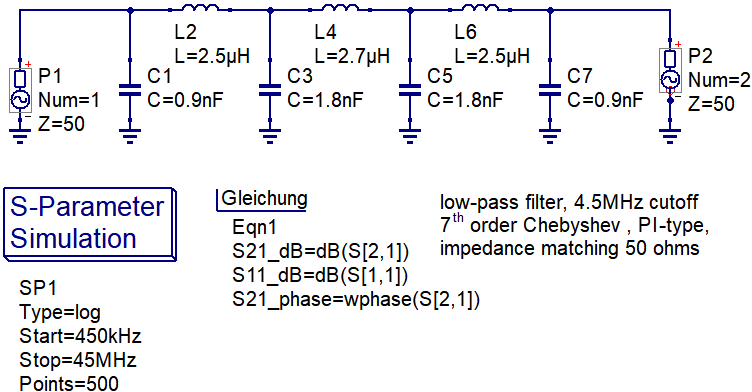
\includegraphics{res/TP_Schaltplan.png}
    \caption{Aufbau des Tschebyscheff-Filters}
\end{figure}

\begin{figure}[H]
    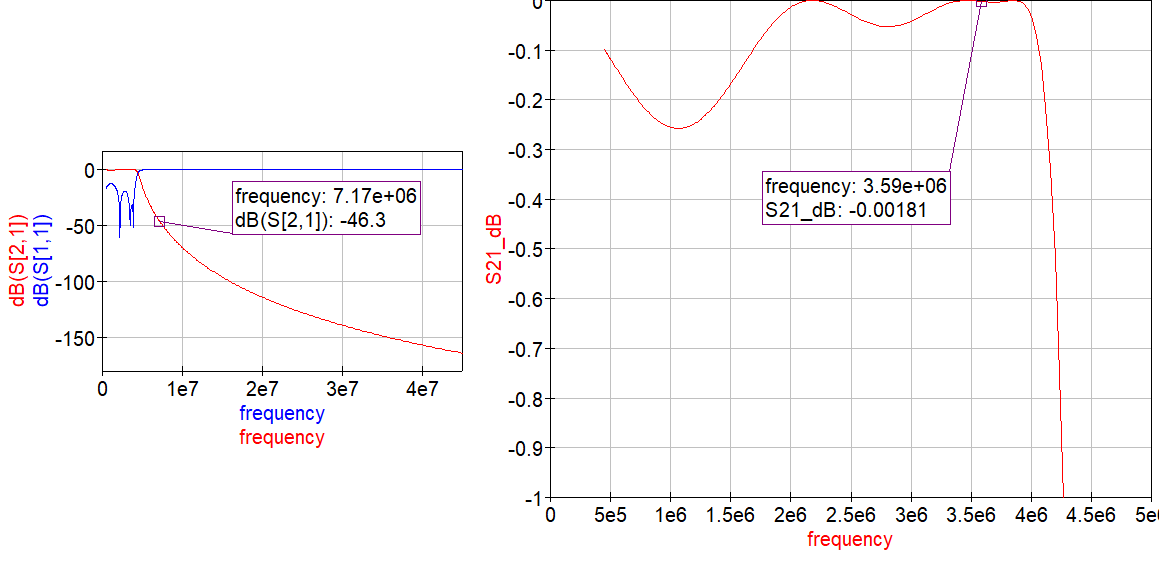
\includegraphics[scale=0.6]{res/TP_Simulation.png}[]
    \caption{Frequenzgang des Filters: Transmission in rot, Reflektionsfaktor in blau}
\end{figure}
Die Simulation zeigt das gewünschte Verhalten des Filters: Bei der gewünschten
Sendefrequenz von [Keine Ahnugn wie viel @TODO] beträgt die Dämpfung quasi $0$dB.
Die für uns eigentlich unkritische Welligkeit bleibt unter $-0.3$dB.